\documentclass{article}
\usepackage[utf8]{inputenc}
\usepackage{natbib}
\usepackage[L7x]{fontenc}
\usepackage[lithuanian]{babel}
\usepackage{lmodern}
\usepackage{amsmath}
\usepackage{graphicx}
\usepackage{framed}
\usepackage{cancel}
\usepackage{tikz}
\usepackage{hyperref}
\usepackage[top=2cm, bottom=2cm, left=1cm, right=1cm, footskip=1cm, a4paper]{geometry}
\def\ph#1{\phantom{#1}}
\begin{document}

\title{Atskliaudimai}
\section*{Gražus paveikslėlis}
Štai gražus paveikslėlis, parodantis lygybę

$$(1+x+x^2+x^3+x^4+x^5)(1+x+x^2+x^3+x^4+x^5)=1+2x+3x^2+4x^3+5x^4+6x^7+5x^8+4x^7+3x^8+2x^9+x^{10}$$

\begin{figure}[ht!]
\centering
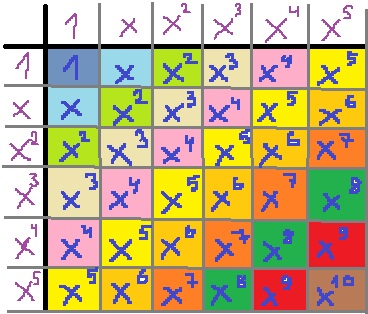
\includegraphics[scale=1.0]{universe}
\label{fig:plytelės}
\end{figure}. 

\section*{Klaidų taisymas}
Pirmą kartą atlikus dauginimus pasimatė daug klaidų, kurias po to daviau ištaisyti (pilka spalva atitinka mokinio variantą, o žalia - kaip teisingai turėtų būti).

\begin{minipage}[b]{0.3\linewidth}
    \begin{itemize}
        \item $(-b)\times (-b) = {\color{black!30}{{(-b)^2}}} = {\color{black!30!green}{b^2}}$
        \item $b\times (-ab) = {\color{black!30}{{-a(b)^2}}} = {\color{black!30!green}{-ab^2}}$
        \item $a\times b^2 = {\color{black!30}{{a(b)^2}}} = {\color{black!30!green}{ab^2}}$
        \item $a^2\times (-b) = {\color{black!30}{{(a^2)(-b)}}} = {\color{black!30!green}{-a^2b}}$
        \item $ab\times (-b) = {\color{black!30}{{a(-b^2)}}} = {\color{black!30!green}{-ab^2}}$
        \item $a\times ab = {\cancel{\color{red}{{a^b}}}} = {\color{black!30!green}{a^2b}}$
     \end{itemize}
\end{minipage}
\hspace{\fill}
\begin{minipage}[b]{0.3\linewidth}
    \begin{itemize}
         \item $-1\times x^3 = {\color{black!30}{-1(x^3)}} = {\color{black!30!green}{-x^3}}$
        \item $-1\times x^2 = {\color{black!30}{-1(x^2)}} = {\color{black!30!green}{-x^2}}$
        \item $-1\times x = {\color{black!30}{-1x}} = {\color{black!30!green}{-x}}$
        \item $2x\times x^2 = {\color{black!30}{2x(x^2)}} = {\color{black!30!green}{2x^3}}$
        \item $-2x\times (-2x) = {\color{black!30}{(-2x)^2}} = {\color{black!30!green}{4x^2}}$
        \item $2\times (-2x) = {\cancel{\color{red}{-4x^2}}} = {\color{black!30!green}{-4x}}$
        \item $a \times (-ab) = {\color{black!30}{(-a^2)b}} = {\color{black!30!green}{-a^2b}}$
    \end{itemize}
\end{minipage}
\hspace{\fill}
\begin{minipage}[b]{0.3\linewidth}
    \begin{itemize}
        \item $a \times (-ca) = {\color{black!30}{(-c(a^2)}} = {\color{black!30!green}{-a^2c}}$
        \item $b \times (-ca) = {\color{black!30}{(-cab)}} = {\color{black!30!green}{-abc}}$
        \item $c \times b^2 = {\color{black!30}{(c(b^2)}} = {\color{black!30!green}{b^2c}}$
        \item $c \times (-bc) = {\color{black!30}{(-b(c^2)}} = {\color{black!30!green}{-bc^2}}$
        \item $c \times (-ca) = {\color{black!30}{((-c^2)a}} = {\color{black!30!green}{-ac^2}}$
        \item $\sqrt{2} \times \sqrt{3} =  {\color{black!30}{\sqrt{2}\sqrt{3}}} = {\color{black!30!green}{-\sqrt{6}}}$ (pagal 8 klasės programą)
    \end{itemize}
\end{minipage}
\section*{Patikslinimai}
\textit{Atsižvelgiant į padarytas klaidas, įvardysiu dauginimo atlikimo taisykles, kuriomis remiantis turėtų išnykti klaidos}
\newline
\begin{framed}
Vienanaris - reiškinys, kurį sudaro tik dauginamieji, iš kurių kiekvienas yra skaičius, kintamasis arba kintamojo laipsnis. 

\begin{itemize}
    \item Kai dauginame keletą vienanarių, turėtume gauti taip pat vienanarį. Tai yra, tokį reiškinį, kuriame aiškiai matosi skaitinė ir raidinė dalys. Keletas pavyzdžių:
    
    $2x\times (-3y) = -6xy$
    
    $(-x)\times(-x) = (-1) \times x \times (-1)\times x=(-1)\times (-1)\times x \times x = x^2$
    
    Pirmoje lygybėje skaitinė dalis yra $-6$, o raidinė $xy$. Antroje lygybėje skaitinė dalis nerašoma, tačiau lygi 1, o raidinė dalis yra $x^2$. Jei skaitinė dalis būtų $-1$, ji taip pat būtų nerašoma.
    \item Nei skaitinėje, nei raidinėje dalyje tarp dauginamųjų nereikia skliaustų: $-3x \times y^2 = \bcancel{\cancel{-3x(y^2)}}-3xy^2$
    \item Rezultate neturi likti tų pačių kintamųjų:
    $ab\times ab = \bcancel{\cancel{abab}}\text{ }a^2b^2$
    \item Norint, kad aiškiau matytųsi panašieji nariai, patartina raidines dalis rašyti alfabetiškai:
    
    $matematika = \bcancel{\cancel{m^2a^3t^2eik}}\text{ } a^3eikm^2t^2$
\end{itemize}
\end{framed}

\section*{Pratimai}

\begin{minipage}[b]{0.4\linewidth}
\begin{enumerate}
    %pirmas
    \item $(x-2)(x+2) = 
    \begin{array}{c||c|c}
     & x & -2 \\
     \hline
     x & \ph{x^2} & \ph{-2x} \\
     \hline
     2 & \ph{2x} & \ph{-4}
     \end{array} = 
     \ph{x^2-2x+2x-4}=\ph{x^2-4}$
     
     %antras
     \item $(x+2)(x+2) = 
    \begin{array}{c||c|c}
     & x & 2 \\
     \hline
     x & \ph{x^2} & \ph{2x} \\
     \hline
     2 & \ph{2x} & \ph{4}
     \end{array} = 
     \ph{x^2+2x+2x+4}=\ph{x^2+4x+4}$
     
     %trečias
     \item $(x-\sqrt{3})(x+\sqrt{3}) = 
    \begin{array}{c||c|c}
     & x & -\sqrt{3} \\
     \hline
     x & \ph{x^2} & \ph{-x\sqrt{3}} \\
     \hline
     \sqrt{3} & \ph{x\sqrt{3}} & \ph{-3}
     \end{array} = 
     \ph{x^2 - 3}$
     
     %ketvirtas
     \item $(x-3)(x+3) = 
    \begin{array}{c||c|c}
     & x & -3 \\
     \hline
     x & \ph{x^2} & \ph{-3x} \\
     \hline
     3 & \ph{3x} & \ph{-9} 
     \end{array} = 
     \ph{x^2-9}$
     
      %penktas
     \item $(a-b)(a-b) = 
    \begin{array}{c||c|c}
     & a & -b \\
     \hline
     a & \ph{a^2} & \ph{-ab} \\
     \hline
     -b & \ph{-ab} & \ph{b^2}
     \end{array} = 
     \ph{a^2-2ab+b^2}$
     \end{enumerate}
     \end{minipage}
\hspace{\fill}
\begin{minipage}[b]{0.5\linewidth}
\subsection*{Sprendimo pavyzdys prisiminimui}
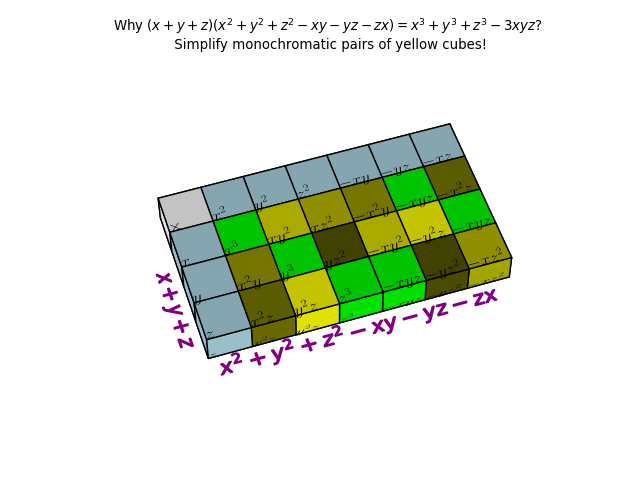
\includegraphics[width=\textwidth]{recipe}
 \end{minipage}
     \begin{enumerate}
     \setcounter{enumi}{5}
     %šeštas
     \item $(a+b)(a-b) = 
    \begin{array}{c||c|c}
     & a & b \\
     \hline
     a & \ph{a^2} & \ph{ab} \\
     \hline
     -b & \ph{-ab} & \ph{-b^2}
     \end{array} = 
     \ph{a^2-b^2}$
     
     %septintas
     \item $(a+b)(a+b) = 
    \begin{array}{c||c|c}
     & a & b \\
     \hline
     a & \ph{a^2} & \ph{ab} \\
     \hline
     b & \ph{ab} & \ph{b^2}
     \end{array} = 
     \ph{a^2+2ab+b^2}$
     
     %aštuntas (kubų sumos formulė)
     \item $(a+b)(a^2-ab+b^2) = 
    \begin{array}{c||c|c}
     & a & b \\
     \hline
     a^2 & \ph{a^3} & \ph{a^2b} \\
     \hline
     -ab & \ph{-a^2b} & \ph{-ab^2} \\
     \hline
     b^2 & \ph{ab^2} & \ph{b^3}
     \end{array} = 
     \ph{a^3+b^3}$
     
     %devintas (kubų skirtumo formulė)
     \item $(a-b)(a^2+ab+b^2) = 
    \begin{array}{c||c|c}
     & a & -b \\
     \hline
     a^2 & \ph{a^3} & \ph{{\color{red}{-a^2b}}} \\
     \hline
     ab & \ph{{\color{red}{a^2b}}} & \ph{{\color{green}{-ab^2}}} \\
     \hline
     b^2 & \ph{{\color{green}{ab^2}}} & \ph{-b^3}
     \end{array} = 
     \ph{a^3-b^3}$
     
     %dešimtas
     \item $(x-1)(x^3+x^2+x+1) = 
    \begin{array}{c||c|c}
     & x & -1 \\
     \hline
     x^3 & \ph{x^4} & \ph{-x^3} \\
     \hline
     x^2 & \ph{x^3} & \ph{-x^2} \\
     \hline
     x & \ph{x^2} & \ph{-x} \\
     \hline
     1 & \ph{x} & \ph{-1}
     \end{array} = 
     x^4-1$
     
     %vienuoliktas
     \item $(x^2-2x+2)(x^2+2x+2) = 
    \begin{array}{c||c|c|c}
     & x^2 & -2x & 2 \\
     \hline
     x^2 & \ph{x^4} & \ph{-2x^3 }& \ph{2x^2} \\
     \hline
     2x & \ph{2x^3} & \ph{4x^2} & \ph{4x} \\
     \hline
     2 & \ph{2x^2} & \ph{-4x^2} & \ph{4} \\
     \end{array} = 
     \ph{x^4+4}$
     
     %dvyliktas
     \item $(a^2+b^2+c^2-ab-bc-ca)(a+b+c) = 
    \begin{array}{c||c|c|c|c|c|c}
     & a^2 & b^2 & c^2 & -ab & -bc & -ca \\
     \hline
     a & \ph{a^3} & \ph{ab^2} & \ph{ac^2} & \ph{-a^2b} & \ph{-abc} & \ph{-a^2c}\\
     \hline
     b & \ph{a^2b} & \ph{b^3} & \ph{c^2 b} & \ph{-ab^2} & \ph{-ab^2} & \ph{-abc}\\
     \hline
     c & \ph{a^2 c} & \ph{b^2c} & \ph{c^3} & \ph{-abc} & \ph{-bc^2} & \ph{-ac^2}
     \end{array} = 
     \ph{a^3+b^3+c^3-3abc}$
     
     %tryliktas 
     \item $(\sqrt{3}+\sqrt{2})(\sqrt{3}-\sqrt{2}) = 
    \begin{array}{c||c|c}
     & \sqrt{3} & \sqrt{2} \\
     \hline
     \sqrt{3} & \ph{3} & \ph{\sqrt{6}} \\
     \hline
     -\sqrt{2} & \ph{-\sqrt{6}} & \ph{-2}
     \end{array} = 
     \ph{3 - 2} = 1$
\end{enumerate}
\section*{Papildomos subtilybės}
Veiksmus taip pat galima atlikti ir trimatėje erdvėje. Kairėje pusėje pademonstruotas projekte \href{https://github.com/loijord/numpyviz/}{\textit{\textbf{numpyviz}}} pavyzdyje nr. 9 yra siūlomas toks skaičiaus $a+b$ kėlimo kvadratu būdas. Ar įstengtumėte atlikti du pratimus dešinėje pusėje?

\begin{minipage}[b]{0.45\linewidth}
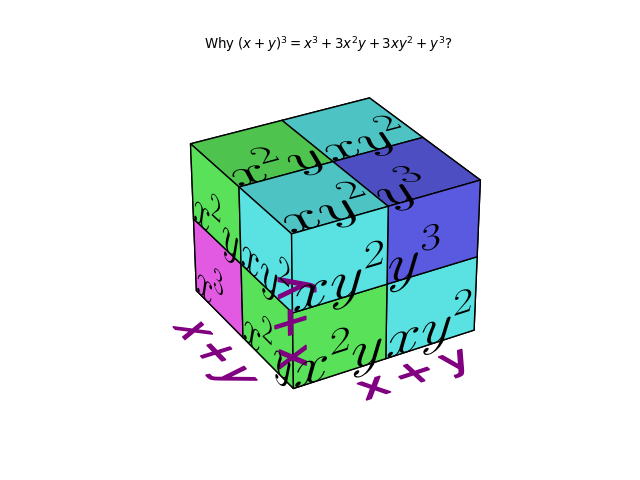
\includegraphics[width=\textwidth]{recipe3}
\end{minipage}
\hspace{\fill}
\begin{minipage}[b]{0.35\linewidth}
\begin{enumerate}
\item $(a-b)(a+b)(a^2+b^2) = 
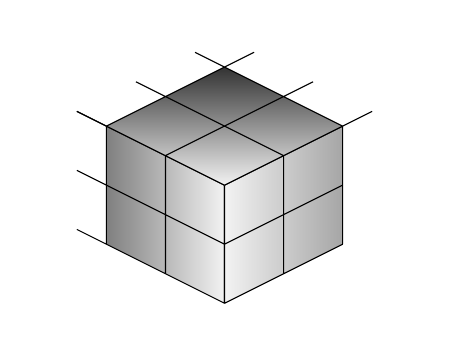
\begin{tikzpicture}[every node/.style={minimum size=1cm}, scale=0.75, baseline=(current bounding box.center)]
\% KAIRYS ŠONAS
\begin{scope}[every node/.append style={yslant=-0.5},yslant=-0.5]
  \shade[right color=gray!10, left color=black!50] (1,1) rectangle +(2,2);
  \node at (0.5,2.5) {};
  \node at (1.5,2.5) {};
  \node at (2.5,2.5) {};
  \node at (0.5,1.5) {};
  \node at (1.5,1.5) {};
  \node at (2.5,1.5) {};
  \draw (0.5,1) grid (3,3);
\end{scope}
\% DEŠINYS ŠONAS
\begin{scope}[every node/.append style={yslant=0.5},yslant=0.5]
  \shade[right color=gray!70,left color=gray!10] (3,-2) rectangle +(2,2);
  \node at (3.5,-0.5) {};
  \node at (4.5,-0.5) {};
  \node at (3.5,-1.5) {};
  \node at (4.5,-1.5) {};
  \draw (3,-2) grid (5,0);
\end{scope}
\% VIRŠUS
\begin{scope}[every node/.append style={yslant=0.5,xslant=-1},yslant=0.5,xslant=-1]
  \shade[bottom color=gray!10, top color=black!80] (5,2) rectangle +(-2,-2);
  \node at (3.5,2.5) {};
  \node at (3.5,1.5) {};
  \node at (3.5,0.5) {};
  \node at (4.5,2.5) {};
  \node at (4.5,1.5) {};
  \node at (4.5,0.5) {};
  \node at (5.5,1.5) {};
  \node at (5.5,0.5) {};
  \draw (3,0) grid (5.5,2.5);
\end{scope}
\end{tikzpicture} = $

\item $(a-b)(a-b)(a-b) = 
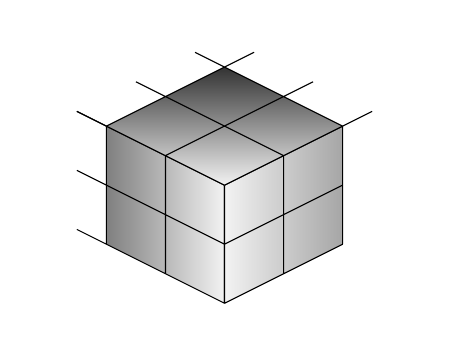
\begin{tikzpicture}[every node/.style={minimum size=1cm}, scale=0.75, baseline=(current bounding box.center)]
\% KAIRYS ŠONAS
\begin{scope}[every node/.append style={yslant=-0.5},yslant=-0.5]
  \shade[right color=gray!10, left color=black!50] (1,1) rectangle +(2,2);
  \node at (0.5,2.5) {};
  \node at (1.5,2.5) {};
  \node at (2.5,2.5) {};
  \node at (0.5,1.5) {};
  \node at (1.5,1.5) {};
  \node at (2.5,1.5) {};
  \draw (0.5,1) grid (3,3);
\end{scope}
\% DEŠINYS ŠONAS
\begin{scope}[every node/.append style={yslant=0.5},yslant=0.5]
  \shade[right color=gray!70,left color=gray!10] (3,-2) rectangle +(2,2);
  \node at (3.5,-0.5) {};
  \node at (4.5,-0.5) {};
  \node at (3.5,-1.5) {};
  \node at (4.5,-1.5) {};
  \draw (3,-2) grid (5,0);
\end{scope}
\% VIRŠUS
\begin{scope}[every node/.append style={yslant=0.5,xslant=-1},yslant=0.5,xslant=-1]
  \shade[bottom color=gray!10, top color=black!80] (5,2) rectangle +(-2,-2);
  \node at (3.5,2.5) {};
  \node at (3.5,1.5) {};
  \node at (3.5,0.5) {};
  \node at (4.5,2.5) {};
  \node at (4.5,1.5) {};
  \node at (4.5,0.5) {};
  \node at (5.5,1.5) {};
  \node at (5.5,0.5) {};
  \draw (3,0) grid (5.5,2.5);
\end{scope}
\end{tikzpicture} = $
\end{enumerate}
\end{minipage}
\hspace{\fill}
\begin{minipage}[b]{0.2\linewidth}
\end{minipage}
\end{document}
